\documentclass[varwidth=true, border=2pt]{standalone}
\usepackage{amsmath,amssymb}% math symbols / fonts
\usepackage{tikz}
\usetikzlibrary{patterns}

\begin{document}
    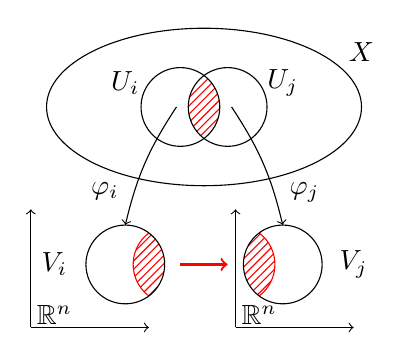
\begin{tikzpicture}
        \draw (0,0) ellipse (2cm and 1cm);
        \begin{scope}[xshift=-2.2cm,yshift=-2.8cm]
            \draw[->] (0,0) -- (0,1.5);
            \draw[->] (0,0) -- (1.5,0);
            \node at (0.3,0.16) {$\mathbb{R}^n$};
        \end{scope}
        \begin{scope}[xshift=0.4cm,yshift=-2.8cm]
            \draw[->] (0,0) -- (0,1.5);
            \draw[->] (0,0) -- (1.5,0);
            \node at (0.3,0.16) {$\mathbb{R}^n$};
        \end{scope}
        \def\ringa{(-0.3,0) circle (0.5cm)}
        \def\ringb{(+0.3,0) circle (0.5cm)}

        \begin{scope}[even odd rule]
            \clip \ringa;
            \fill[pattern color=red,pattern=north east lines] \ringb;
        \end{scope}

        \begin{scope}[even odd rule,shift={(-0.7,-2)}]
            \clip \ringa;
            \fill[draw=red,pattern color=red,pattern=north east lines] \ringb;
        \end{scope}

        \begin{scope}[even odd rule,shift={(+0.7,-2)}]
            \clip \ringb;
            \fill[draw=red,pattern color=red,pattern=north east lines] \ringa;
        \end{scope}
        \draw \ringa;
        \draw \ringb;

        \node at (-1,0.3) {$U_i$};
        \node at (+1,0.3) {$U_j$};
        \node at (-1.9,-2) {$V_i$};
        \node at (+1.9,-2) {$V_j$};
        \node at (+2.0,0.7) {$X$};

        \path[->] (-0.35,0)  edge [bend angle=10,bend right] node[label={[label distance=0.1cm]210:$\varphi_i$}] {} (-1,-1.5);
        \path[->] (+0.35,0)  edge [bend angle=10,bend left]  node[label={[label distance=0.1cm]-30:$\varphi_j$}] {} (+1,-1.5);

        \draw (-1,-2) circle (0.5cm);
        \draw (+1,-2) circle (0.5cm);

        \draw[->, red, thick] (-0.3,-2) -- (0.3,-2);
    \end{tikzpicture}
\end{document}
